
\item One mole of a monatomic ideal gas undergoes a cyclic process as shown in the figure (where \( V \) is the volume and \( T \) is the temperature). Which of the statements below is (are) true?
    \begin{center}
        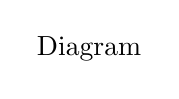
\begin{tikzpicture}
            \node {Diagram};
        \end{tikzpicture}
    \end{center}
    \begin{tasks}(1)
        \task Process I is an isochoric process
        \task In process II, gas absorbs heat
        \task In process IV, gas releases heat
        \task Processes I and III are not isobaric
    \end{tasks}
